La planificación del sistema constituye una fase crítica en el desarrollo del
proyecto. Como se mencionó anteriormente en el punto \ref{sec:rt-analysis}, se
cuentan con múltiples tareas que comparten recursos y que se deben ejecutar
con cierta frecuencia para enviar los datos al servidor remoto y detectar los
eventos que se produzcan en el sistema.

El diagrama esquemático que representa al sistema con sus tareas es:

\begin{figure}[H]
  \centering
  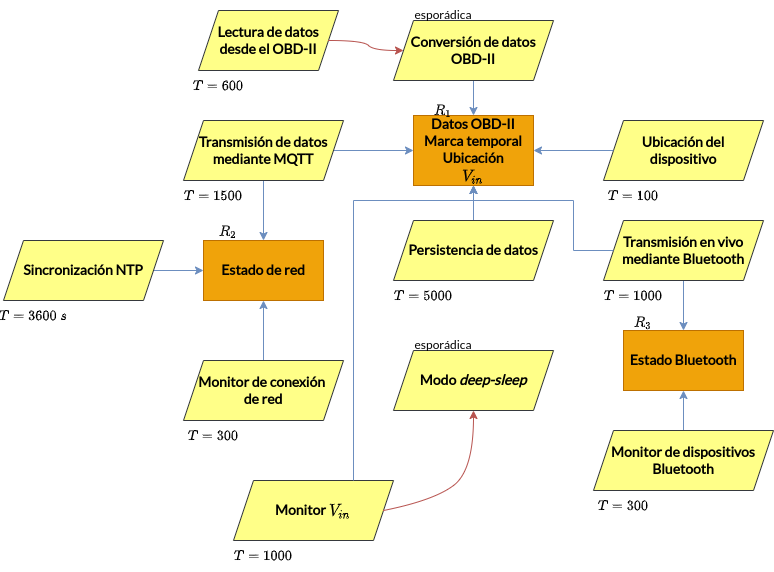
\includegraphics[width=\linewidth]{images/Plannification.png}
  \caption{Diagrama esquemático del sistema con las tareas y objetos protegidos que lo conforman.}
  \label{fig:plannification-diagram}
\end{figure}

En la figura \ref{fig:plannification-diagram} se pueden apreciar las tareas y los
objetos protegidos compartidos por las tareas. En particular, las tareas se representan
por los trapecios amarillos que van acompañados de sus periodos o se indican si son
tareas esporádicas. Los objetos protegidos se representan como rectángulos de color
naranja y se indica, mediante flechas, qué tareas acceden a ellos.

Los datos de las tareas vienen representados en la tabla \ref{tab:rt-table}:

\begin{table}[H]
  \centering
  \begin{tabularx}{\linewidth}{c|X|c|c|c|c|c|c|c}
    $i$  & \textbf{Tarea}                         & \textbf{Tipo} & $T_i~\left(ms\right)$ & $D_i~\left(ms\right)$ & $C_i$    & $R_1$      & $R_2$   & $R_3$      \\
    \hline\hline
    $1$  & Lectura de datos desde \ac{OBD}--II    & $P$           & $600$                 & $400$                 & $C_1$    &            &         &            \\
    $2$  & Conversión de datos \ac{OBD}--II       & $S$           & $700$                 & $200$                 & $C_2$    & $r^2_1$    &         &            \\
    $3$  & Sincronización NTP                     & $P$           & $3.6 \cdot 10^6$      & $1000$                & $C_3$    &            &         &            \\
    $4$  & Transmisión de datos mediante MQTT     & $P$           & $1500$                & $1000$                & $C_4$    & $r^4_1$    & $r^4_2$ &            \\
    $5$  & Ubicación del dispositivo              & $P$           & $100$                 & $100$                 & $C_5$    & $r^5_1$    &         &            \\
    $6$  & Persistencia de datos                  & $P$           & $5000$                & $2000$                & $C_6$    & $r^6_1$    &         &            \\
    $7$  & Transmisión en vivo mediante Bluetooth & $P$           & $1000$                & $500$                 & $C_7$    & $r^7_1$    &         & $r^7_3$    \\
    $8$  & Monitor de conexión de red             & $P$           & $300$                 & $300$                 & $C_8$    &            & $r^8_2$ &            \\
    $9$  & Modo \textit{deep-sleep}               & $S$           & $5000$                & $30000$               & $C_9$    &            &         &            \\
    $10$ & Monitor $V_{in}$                       & $P$           & $1000$                & $100$                 & $C_{10}$ & $r^{10}_1$ &         &            \\
    $11$ & Monitor de dispositivos Bluetooth      & $P$           & $300$                 & $300$                 & $C_{11}$ &            &         & $r^{11}_3$ \\
    \hline
  \end{tabularx}
\end{table}
